\documentclass[11pt,a4paper]{article}
\usepackage{fontspec}
\usepackage[turkish,shorthands=off]{babel}
\setmainfont{Times New Roman}
\setmonofont{Menlo}[Scale=0.85]
\usepackage[margin=2.3cm]{geometry}
\usepackage{amsmath,booktabs,graphicx,xcolor,caption}
\usepackage[hidelinks]{hyperref}
\makeatletter\newcommand\tabin[1]{\@@input #1 }\makeatother
\sloppy
\setlength{\parskip}{0.5em}\setlength{\parindent}{0pt}
\newcommand{\bel}{\textcolor{teal}{\textbf{\footnotesize [belgelenmiş]}}}
\newcommand{\yor}{\textcolor{orange!80!black}{\textbf{\footnotesize [yorum]}}}
\newcommand{\hip}{\textcolor{purple}{\textbf{\footnotesize [hipotez]}}}
\newcommand{\kod}[1]{{\XeTeXinterchartokenstate=0 \texttt{#1}}}

\title{Mac simülasyon koşuları: sonuçlar ve\\ BBA geçiş 2 incelemesi}
\author{Hazırlayan: Claude (Claude Code, Mac oturumu)}
\date{19 Kasım 2026}

\begin{document}
\maketitle

\section*{Kısaca}
\kod{MAC\_PROMPT.md}'deki üç iş Mac'te (M1, 8 çekirdek) eksiksiz bitti ve sonuçları
\kod{claude/brave-allen-92wn61} dalına gönderildi. Yinelemeli (iteratif) BBA, sahte EDM'yi
hedefin 78 katından 0{,}72 katına indirdi (108 kat bastırma). Geçiş 2'de görülen artış
(4{,}17$\times$ $\to$ 13{,}40$\times$) bir bozulma değil: geçiş 1'deki düşük değer, sahte EDM'yi
oluşturan dört kanalın rastlantısal olarak birbirini götürmesinden geliyor. Bunu her geçişin
desenini kanallara ayırıp yeniden ölçerek doğruladım (Bölüm~4). Son geçişlerde (6--8) düşüş yavaşlıyor; kalan sahte EDM tümüyle dx $\times$ dy çarpımından geliyor ve antisimetrik yatay kaçıklık içeren iki kanalda toplanıyor.

Bu raporda üç tür ifade var. \bel\ olanlar doğrudan ölçülen sayılara dayanır,
\yor\ olanlar bu sayılardan çıkardığım sonuçlardır, \hip\ olanlar ise sınanmamış
açıklamalardır.

\section{Ortam ve yapılanlar}
Koşular 18 Kasım 11:58 ile 19 Kasım 00:53 arasında yapıldı. Python için conda ortamı
\kod{ml} (numpy 2.4.6, scipy 1.17.1) kullanıldı; sistemdeki \kod{python3}'te numpy yoktu.
İki C++ motoru (\kod{integrator.dylib} ve \kod{revizyon/integrator.dylib}) Mac'te clang++ ile
yeniden derlendi; bu ikili dosyalar commit edilmedi. Başlangıç commit'i \kod{70c7178}.

Sırasıyla şu işler çalıştı, hepsi 8 işçiyle (\kod{-w 8}) ve birbiri ardına:
\begin{enumerate}
\item \kod{build\_rtrue.py --sig-g 0.002}: \%1 β-beat'li ,,gerçek makine'' tepki matrisleri.
  2 dakika sürdü. Nominal matristen göreli farkları \%1{,}5--1{,}9 arasında; hiçbirinde NaN yok. \bel
\item \kod{makale\_yeniden\_olcum.py}: 74 görevin 74'ü tamam, 26 dakika (tahmin 2 saatti). \bel
\item \kod{classic\_bba\_iter\_donmus.py --passes 8 --bbeat 0.01 --rmatrix cpp}: 12{,}5 saat
  (44\,820 s). Tek gerçekleşme: seed 0, kaçıklık σ = 10 μm. \bel
\end{enumerate}

Sonuçlar şu commit'lerde: \kod{aa23f8b} (yeniden ölçüm), \kod{aef2694} ile \kod{23e0874} arası
(BBA ara ve son durumları).

\section{Makale yeniden ölçümü}
Tablo~\ref{tab:yo}'deki $f^*$ değerleri sahte EDM'nin hedefe oranıdır:
$f^* = f / (10^{-9}\ \text{rad/s})$. Yani $f^*=1$, sahte EDM'nin 1 nrad/s'lik hedefe eşit olduğu
anlamına gelir. ,,Yön'' $-1$ saat yönünün tersini (CCW), $+1$ saat yönünü (CW) gösterir.

\begin{table}[h]\centering\small
\caption{\kod{makale\_yeniden\_olcum.jsonl} özeti (n: seed sayısı).}\label{tab:yo}
\begin{tabular}{lrlrrrr}\toprule
tür & σ (μm) & kanal & yön & n & ortalama $f^*$ & RMS $f^*$\\\midrule
\tabin{tablo_yo.tex}
\bottomrule\end{tabular}\end{table}

Üç gözlem:

\textbf{σ² ölçeklemesi temiz.} Aynı desen (seed 0) σ = 2{,}5 $\to$ 5 $\to$ 10 μm büyütüldüğünde
sa, as ve aa kanallarında $f$ her adımda 4{,}00--4{,}03 kat büyüyor; kaçıklık iki katına çıkınca
etki dört katına çıkıyor. Bu, sahte EDM'nin kaçıklığın karesiyle büyüyen geometrik faz olduğunu
söyleyen beklentiyle uyumlu. En küçük sinyalli ss kanalında oranlar 3{,}79 ve 4{,}09. \bel

\textbf{İki demet düzeltmesi (tb20) iki yönde de küçük:} RMS $f^*$ $\approx$ 0{,}2 (15 seed). \bel

\textbf{Tek demet düzeltmesi (oc1) yöne göre asimetrik:} yön $+1$'in RMS'i yön $-1$'inkinin
yaklaşık 17 katı. \bel\ Bu düzeltmede yalnız CCW tepki matrisi kullanıldığı için
beklenen bir durum olabilir, ama bunu ayrıca sınamadım. \hip

\section{İteratif BBA sonuçları}
Her geçişte BBA kalan kaçıklığı tahmin edip düzeltiyor, ardından sahte EDM donmuş-spin noktasında
ölçülüyor. Tablo~\ref{tab:bba}'daki ,,simetrik'' sütunlar kalan kaçıklığın orbit-kör simetrik
kısmının RMS'idir; ,,yörünge'' dikey kapalı yörüngenin kaba göstergesidir; ,,min.~kalite''
BBA tahmininin en kötü quad'daki güvenilirlik katsayısıdır (1 iyi).

\begin{table}[h]\centering\small
\caption{Geçiş başına BBA sonuçları (ham: 78$\times$ hedef, başlangıç yörünge $\approx$48 μm).}\label{tab:bba}
\begin{tabular}{rrrrrc}\toprule
geçiş & $|f|$/hedef & sim.~dx (μm) & sim.~dy (μm) & yörünge (μm) & min.~kalite x/y\\\midrule
\tabin{tablo_bba.tex}
\bottomrule\end{tabular}\end{table}

Kalan simetrik kaçıklık ve yörünge her geçişte düzenli küçülüyor: dy 3{,}27 μm'den 0{,}057
μm'ye, dx 4{,}27 μm'den 0{,}90 μm'ye, yörünge 24{,}9 μm'den 1{,}0 μm'ye. \bel\ Yatay düzlem
belirgin biçimde daha yavaş yakınsıyor; yatay tahmin kalitesi ilk geçişlerde düşük (0{,}10)
ve ancak 8. geçişte 0{,}70'e çıkıyor. \bel\ Buna karşılık sahte EDM düzgün inmiyor:
4{,}17 $\to$ 13{,}40 $\to$ 9{,}60 $\to$ 4{,}37 $\to$ 0{,}01 $\to$ 1{,}21 $\to$ 1{,}09 $\to$ 0{,}72.
Bir sonraki bölüm bu iniş-çıkışın nedenini açıklıyor.

\section{Geçiş 2'de sahte EDM neden arttı?}
\subsection*{Fikir: sahte EDM dört kanalın toplamı}
Kaçıklık desenini iki parçaya ayırabiliriz. Bir FODO hücresindeki iki quad'ın (QF ve QD)
kaçıklıkları aynı yöndeyse buna simetrik (s), zıt yöndeyse antisimetrik (a) kısım denir.
Simetrik kısım kapalı yörüngede neredeyse görünmez, antisimetrik kısım görünür. Bu ayrımı hem
yatay (dx) hem dikey (dy) kaçıklık için yaparsak dört eşleşme çıkar: ss, sa, as, aa. Burada ilk
harf dx'in, ikinci harf dy'nin parçasıdır.

Sahte EDM, kabaca dx ile dy'nin çarpımıyla oluşur (bilineer):
\[
 f \approx \mathbf{dx}^{\mathsf T} M\, \mathbf{dy}.
\]
Burada $\mathbf{dx}$ ve $\mathbf{dy}$ 48 quad'ın kaçıklıklarını tutan vektörler (metre),
$M$ makinenin optiğinden gelen sabit bir matris, $f$ ise sahte EDM'dir (rad/s). Her vektörü
$\mathbf{dx} = \mathbf{dx}_s + \mathbf{dx}_a$ diye ikiye ayırıp çarpımı açınca
\[
 f = f_{ss} + f_{sa} + f_{as} + f_{aa}
\]
elde edilir. Önemli nokta şu: bu dört terimin işaretleri birbirinden bağımsızdır. Biri pozitif,
öbürü negatif olabilir; o zaman toplam, terimlerin tek tek büyüklüğünden çok daha küçük çıkar.

Bu ayrıştırmanın simülasyonda gerçekten geçerli olduğunu sınadım. Geçiş 0'da (düzeltme öncesi)
kanallar $-4{,}89$, $+35{,}44$, $-80{,}53$ ve $+127{,}89$; toplamları $77{,}91$. Tam desen için
ayrı ölçülen değer de $77{,}91$. Fark ölçüm hassasiyetinin altında. \bel

\subsection*{Ölçüm}
Her geçişin kalan desenini (\kod{res\_x}, \kod{res\_y}) dört kanala ayırıp sahte EDM'yi
\emph{işaretiyle} yeniden ölçtüm. Ayar BBA ile aynı: \kod{measure\_frozen}, CCW, 28 tur,
4 yineleme. BBA betiği yalnız $|f|$ kaydettiği için işaret orada görünmüyordu.
Betik: \kod{bba\_kanal.py}, veri: \kod{revizyon/sonuclar/bba\_gecis\_kanallar.jsonl}.

\begin{table}[h]\centering\small
\caption{Kanallara ayrılmış sahte EDM ($f^*$, işaretli). ,,Σ'': dört kanalın toplamı.
,,Sönüm'': $\sum|f_{ij}| / |f|$; 1'e yakınsa kanallar aynı yönde, büyükse birbirini götürüyor.}\label{tab:kanal}
\begin{tabular}{rrrrrrrr}\toprule
geçiş & ss & sa & as & aa & tam ($f$) & Σ & sönüm\\\midrule
\tabin{tablo_kanal.tex}
\bottomrule\end{tabular}\end{table}

\begin{figure}[h]\centering
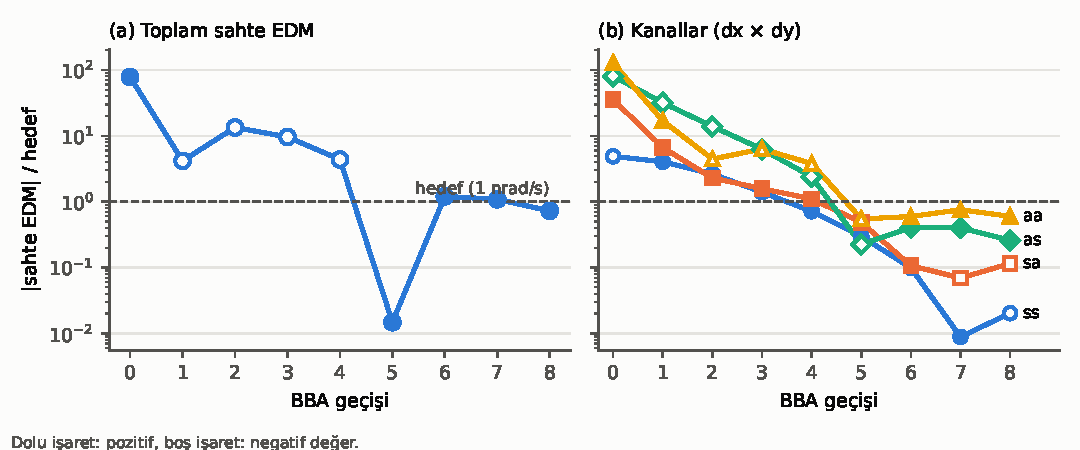
\includegraphics[width=\linewidth]{bba_kanallar.pdf}
\caption{(a) Toplam sahte EDM ve (b) dört kanalın büyüklüğü, geçişe göre (log ölçek).
Kesikli çizgi 1 nrad/s hedefi. Geçiş 1, 2 ve 5'teki iniş-çıkışlar kanalların birbirini götürmesinden; geçiş 6'dan sonra as ve aa işaret değiştirip $\approx$0,3--0,8 düzeyinde kalıyor.}
\label{fig:kanal}\end{figure}

\subsection*{Ne oldu?}
Geçiş 1'den 2'ye sayılar şöyle değişiyor (Tablo~\ref{tab:kanal}): \bel
\begin{itemize}
\item as kanalı (antisimetrik dx $\times$ simetrik dy) en büyük kanal: $-31{,}76$ $\to$
  $-13{,}89$. Yani 2{,}3 kat \emph{küçüldü}.
\item aa kanalı $+16{,}91$ $\to$ $-4{,}44$: küçüldü ve \emph{işaret değiştirdi}.
\item ss ($+4{,}04 \to +2{,}63$) ve sa ($+6{,}65 \to +2{,}29$) de küçüldü.
\end{itemize}

Geçiş 1'de toplam şöyle oluşuyor: $4{,}04 + 6{,}65 - 31{,}76 + 16{,}91 = -4{,}17$. Büyüklükleri
toplamı 59{,}4 olan dört terim, birbirini götürerek yalnız 4{,}17 bırakıyor; sönüm oranı $\approx$14.
Geçiş 2'de aa işaret değiştirince as'ı artık götürmüyor, tersine ona ekleniyor:
$2{,}63 + 2{,}29 - 13{,}89 - 4{,}44 = -13{,}40$. Sönüm oranı 1{,}7'ye düşüyor.

Kısacası geçiş 2'de her kanal küçüldü; toplam büyüdü, çünkü geçiş 1'deki rastlantısal götürme
ortadan kalktı. Geçiş 1'deki 4{,}17$\times$ değeri iyimser bir rastlantıydı. BBA'nın
gerçek ilerlemesini ilk geçişlerde daha dürüst gösteren sayı, baskın kanalın büyüklüğüdür:
as kanalı geçiş 4'e kadar 80{,}5 $\to$ 31{,}8 $\to$ 13{,}9 $\to$ 6{,}3 $\to$ 2{,}4; her geçişte
yaklaşık 2{,}3 kat küçülüyor. \bel

Aynı rastlantı geçiş 5'te ters yönde görülüyor: kanallar $+0{,}30$, $+0{,}49$, $-0{,}22$ ve
$-0{,}55$ iken toplam yalnız $+0{,}015$ (sönüm $\approx$100). O geçişteki 0{,}01$\times$ da gerçek bir
bastırma değil, sıfır geçişine yakın düşmüş bir değer. \bel\ (sayılar) / \yor\ (yorum)

\subsection*{Son geçişler (5--8): düşüş yavaşlıyor}
Geçiş 6'da as ve aa kanalları işaret değiştiriyor ve sonra küçülmeyi büyük ölçüde bırakıyor:
aa $+0{,}60 \to +0{,}75 \to +0{,}60$, as $+0{,}41 \to +0{,}40 \to +0{,}26$ (geçiş 6, 7, 8). \bel\
Bu geçişlerde sönüm oranı 1{,}0--1{,}4; yani kanallar artık aynı yönde ve son değer
0{,}72$\times$ bir rastlantı değil, gerçek bir kalıntıdır. \yor

Kalan sahte EDM'yi taşıyan iki kanal (as ve aa) ortak bir özelliğe sahip: ikisinde de dx'in
\emph{antisimetrik} kısmı var. Simetrik dx 0{,}90 μm ile antisimetrik dx'ten (0{,}70 μm) büyük
olduğu halde, simetrik dx içeren ss ($-0{,}02$) ve sa ($-0{,}11$) kanalları küçük. \bel\
Antisimetrik kaçıklık kapalı yörüngede büyük iz bırakır; sahte EDM de kapalı yörüngenin
çarpımından ($x_{CO}\cdot y_{CO}$) geldiği için bu beklenen bir şey. \yor

\textbf{Bir taban mı var?} Bilineer modelde aa kanalı, antisimetrik dx ile antisimetrik dy'nin
RMS çarpımıyla birlikte küçülmeli. Bu çarpım geçiş 6, 7, 8'de $0{,}933 \times 0{,}154 = 0{,}144$,
$0{,}800 \times 0{,}085 = 0{,}068$ ve $0{,}702 \times 0{,}048 = 0{,}034$ μm²; her geçişte yarıya
iniyor. aa ise neredeyse sabit. \bel\ Bu iki şeyle açıklanabilir: ya dx'e ya da dy'ye tek başına
bağlı, çarpım olmayan bir taban vardır; ya da çarpım hâlâ geçerlidir ama desenin şekli değişiyordur.

Ayırmak için geçiş 8 desenini altı biçimde yeniden ölçtüm (Tablo~\ref{tab:taban}). Bir terim
saf çarpımsa dy sıfırlanınca kaybolmalı ve dy'nin işareti ters çevrilince kendisi de işaret
değiştirmelidir.

\begin{table}[h]\centering\small
\caption{Geçiş 8 deseninde bilineerlik testi ($f^*$). Veri:
\kod{revizyon/sonuclar/bba\_gecis8\_taban.json}.}\label{tab:taban}
\begin{tabular}{lr}\toprule
desen & $f^*$\\\midrule
aa: ($P_a$dx, $P_a$dy) & $+0{,}599$\\
aa, dy işareti ters & $-0{,}600$\\
aa, dy = 0 & $+0{,}002$\\
aa, dx = 0 & $+0{,}002$\\
tam desen (dx, dy) & $+0{,}724$\\
tam desen, dy işareti ters & $-0{,}728$\\
tam desen, dy = 0 & $+0{,}002$\\
\bottomrule\end{tabular}\end{table}

Sonuç açık: tek başına dx'e ya da dy'ye bağlı katkı yalnız $\approx$0{,}002 (hedefin binde ikisi), dy
ters çevrilince sonuç tam işaret değiştiriyor. Kalan sahte EDM \emph{tümüyle} dx $\times$ dy
çarpımından geliyor; taban yok. \bel\ Dolayısıyla aa'nın küçülmemesi desenin şekliyle ilgili:
,,aa / (RMS çarpımı)'' oranı geçiş 6'da 4{,}2, geçiş 8'de 17{,}8 μm$^{-2}$. \bel\ Benim tahminim
şu: BBA, dy'nin dx ile zayıf eşleşen bileşenlerini hızlı, güçlü eşleşen bileşenlerini yavaş
düzeltiyor; böylece kalan dy giderek sahte EDM'ye en çok katkı veren biçimlerde toplanıyor. \hip\
Bunu sınamak için kalan dy'nin harmonik (Fourier) içeriğine geçiş geçiş bakmak gerekir; yapmadım.

\subsection*{Dikkat çeken iki ayrıntı}
\textbf{aa kanalı geçiş 2--3'te büyüyor} ($|{-4{,}44}| \to |{-6{,}30}|$), sonra yeniden
küçülüyor. \bel\ Muhtemel neden yatay tahminin bu geçişlerde düşük kaliteli olması
(min.~kalite x 0{,}18--0{,}28): yatay düzeltme kısılınca antisimetrik dx yavaş değişirken dikey
düzeltme dy'yi hızla değiştiriyor ve aa'nın işaretli değeri sıfırdan geçip öbür yanda
büyüyebiliyor. \hip

\textbf{ss kanalı geçiş 1'de işaret değiştiriyor} ($-4{,}89 \to +4{,}04$). \bel\ Simetrik
kısmın bu geçişte hedefi aştığını (overshoot) düşündürüyor; sonraki geçişlerde aynı işaretle
düzgün küçülüyor. \hip

\section{Sonuç ve öneriler}
\begin{enumerate}
\item Geçiş 2'deki artış BBA'nın bozulması değil; kanalların rastlantısal birbirini götürmesinin
  kalkmasıdır. Her kanal o geçişte küçüldü. \yor
\item Tek bir gerçekleşmede, tek bir geçişin $|f|$ değeri bu yüzden çok oynak: aynı ilerleme
  düzeyinde 0{,}01$\times$ de 13$\times$ da çıkabiliyor. Makalede ,,$N$ geçişten sonra
  sahte EDM şu kadar'' demek için ya birden çok seed'in RMS'i, ya da kanal büyüklüklerinin
  toplamı ($\sum|f_{ij}|$, en kötü durum sınırı) daha güvenilir bir ölçü olur. \yor
\item 8 geçiş sonunda $|f| = 0{,}72\times$ hedef. Bu son değerde sönüm küçük (1{,}4; kanal
  büyüklükleri toplamı 0{,}99), yani rastlantıyla küçülmüş bir sayı değil. Ama tek seed'lik. \bel
\item Geçiş 6'dan sonra düşüş yavaşlıyor: hedefin $\approx$1 katı civarında, 3 geçişte yalnız 1{,}21
  $\to$ 0{,}72. Kalıntıyı antisimetrik dx içeren as ve aa kanalları taşıyor; tek başına dx'e ya
  da dy'ye bağlı bir taban yok (Tablo~\ref{tab:taban}). \bel
\item Yavaşlamanın nedeni büyük olasılıkla kalan desenin şekli: dy'nin sahte EDM'ye en çok katkı
  veren bileşenleri en yavaş düzeliyor. \hip\ Sınamak için kalan dy'nin harmonik içeriği
  geçiş geçiş incelenebilir.
\item BBA yatay düzlemde dikeyden belirgin biçimde yavaş yakınsıyor (sim.~dx 0{,}90 μm, dy
  0{,}057 μm; yatay tahmin kalitesi ilk geçişlerde 0{,}10). Daha fazla geçiş ya da yatayda daha
  yüksek gevşeme katsayısı kalıntıyı azaltabilir. \hip
\end{enumerate}

\section{Anormallikler ve notlar}
\begin{itemize}
\item \kod{makale\_yeniden\_olcum.py} tahmin edilen 2 saat yerine 26 dakikada bitti; 74/74 görev
  tamam, günlükte hata yok. \bel
\item Zincir betiğindeki otomatik commit ilk iki seferde çalışmadı: \kod{git add} listesinde henüz
  var olmayan dosyalar vardı. O commit'ler elle atıldı; sonraki 2 saatlik commit'ler düzgün
  çalıştı. Veri kaybı yok. \bel
\item 18 Kasım 13:45'te e-posta taraması (yerel Qwen 9B) BBA ile aynı anda çalıştı ve $\approx$1{,}5 saat
  işlemciyi paylaştı; kullanıcı isteğiyle 15:20'de durduruldu. BBA hatasız sürdü; geçiş 1 ve 2 yaklaşık aynı sürede ($\approx$90 dk) bitti, belirgin bir yavaşlama görülmedi. \bel
\item Kanal ayrıştırması için ek olarak 45 \kod{measure\_frozen} çağrısı (9 geçiş × 5 kanal), bilineerlik testi için 6 çağrı daha yapıldı (düşük
  öncelikle, BBA ile paralel). \bel
\end{itemize}

\end{document}
